\newcommand{\archid}{1}
\chapter{Design of WSN monitoring platform architecture}
\label{ch:architecture}
%What needs to be monitored: sensor-networks/IoT
%How data and information streams flow and combine
%will focus on data sources and streams as to ascertain which architecture, configuration and components are needed/suitable.
This chapter will detail the process taken in order to device the platform and its architecture. This will be accomplished by first exploring the general problem domain. Subsequently, the design of the proposed platform and its implementation will be deliberated by identifying the available supporting technologies, clarifying the adaptations made to those technologies and explaining further implementation details. The chapter will be concluded by discussing the advantages, limitations and considerations of the proposed solution.
\section{Objective of this chapter}
Large sensor applications send immense amounts of low-level raw monitoring data that requires capturing, enriching and processing. Individual snapshots of raw data will contain very little information. However, when accumulated, these snapshots contain the potential from which meaningful conclusions can be derived. These decisions range from single sensor scale to the sensor application as a whole. The raw data is enriched by combining and analysing datasets of similar, related data, in order to achieve a higher degree of information.

The objective of the efforts described in this chapter is to conceive a software platform that enables software developers to construct their own sensor application monitoring system. The intention to achieve this is by devising a generic application backbone and base building blocks for  developers to compose and extend.
\section{Conceptualization of the problem domain}
In this section the problem domain will be investigated in order to eventually determine the requirements for the model. This will achieved by performing a commonality/variability analysis (C/V analysis) of the problem domain, as described in Section \ref{sec:back:cv_analysis}. The analysis consists of three concepts:
\begin{itemize}
\nospace
\item The definitions that will be used in the analysis and the remainder of this chapter,
\item the common features shared by all elements in the problem domain and which may be assumed as established concepts, and
\item the variations that appear between aspects of the problem domain for which must be accounted for in the proposed solution.
\end{itemize}
\subsubsection*{Definitions}
Firstly, some key terms will be defined that will be used in the analysis and the remainder of this chapter.
\begin{description}[style=nextline]
\nospace
\item[Platform] The monitoring platform to be designed.
\item[Application] The application that is being investigated by the platform.
\item[Snapshot] A message containing a collection of data points indicating the state of a system on a certain instant.
\item[Source] An entity emitting a snapshot. This can be a physical end-device, external service or an process internal to the platform.
\item[Consequence] An action effected by the platform based on the analysis of one or more snapshots.
\end{description}
\subsubsection*{Commonalities}
With the definitions established some common features shared by each application in the problem domain will be identified next. These commonalities may be presumed during the design of the platform and grants a scope to the design efforts.
\begin{enumerate}[label=C\archid .\arabic*]
\nospace
\item \label{c:scale_sensor} The group of target applications involves an enormous amount of sensors, which entails a high throughput of snapshots requiring analysis by the platform.
\item \label{c:snapshot} As mentioned in the definitions, data is captured in snapshots. These represent the (partial) state of the application as measured or determined at a certain point in time. These snapshots can be used for both input of the platform as for representing intermediary computation states.
\item \label{c:snapshot_transformation} The parameters and values of a snapshot, and therefore consecutive derived values, may be considered fixed. Parameters can only change by outputting a new snapshot, not during evaluation of the current one.
\end{enumerate}
\subsubsection*{Variabilities}
Finally, the variety within the problem domain will be explored. As the purpose of the solution is to process information, the analysis will mostly focus on the variations in the domain of data and information produced by applications. The solution should provide proficient adaptability in order to account for these variabilities. This will be ensured by captivating these variations in requirements.
\begin{enumerate}[label=V\archid .\arabic*]
\nospace
\item \label{v:qoi} The first variety  encountered is the variation in Quality of Information (QoI). As described in the Background chapter (section \ref{sec:back:qoi}), there are many parameters characterizing the QoI of data. A snapshot or collection of snapshots can vary on any combination of them.
\item \label{v:conclusion_basis} Secondly, there is the information base on which conclusions are made. The first conclusion basis is elementary:
\begin{enumerate}
\nospace
\item Single snapshot. (e.g. a sensor requiring maintenance)
\end{enumerate}
The second identified analysis is based on a large amount of low-information snapshots \cite{qos_difficult}, of which two types are identified:
\begin{enumerate}[resume]
\nospace
\item Multiple sequentially relevant snapshots from a single source (longitudinal), used to analyse tendency of parameters. (e.g. a sharp continuous increase in bandwidth used may indicate future capacity issues.)
\item Many multi-source snapshots without individual significance (lateral). E.g: while the individual bandwidth usage of sensors may be of little interest, knowledge of the average and total bandwidth usage of the system may be warranted.
\end{enumerate}
\item \label{v:consequence} The possible consequences by the platform have a large range of implementations and cannot be fully anticipated. However, though the exact implementation of consequences can never be anticipated exactly, some groups of consequences can be identified.
\begin{enumerate}
\nospace
\item Build a model for reporting purposes. In order to generate reports some high-level information data points need to be calculated based on large datasets. These data points are then exposed either by an in-memory component with an API or by persisting it to intermediary permanent storage.
\item Analyses which invoke immediate responses to the application or a command \& control service administrating the application.
\item Alerting or reporting according to a specified rule. When this user defined rule is met or violated an alert is sent to a maintenance operator or auxiliary system.
\end{enumerate}
\end{enumerate}
The final variety is the scale of the application. It has already been established that the platform will operate on applications of very large-scale, i.e. thousands of sensors. However, given a thousand as lower bound, the upper bound is still uncertain. Therefore, the size of the application is still uncertain and differing degrees of size require different computational needs.
\begin{enumerate}[label=V\archid .\arabic* , resume]
\nospace
\item \label{v:scale} The scale of large wireless sensor applications varies wildly. This yields for both the number of devices in the application and the rate at which a device emits snapshots.
\end{enumerate}
\section{Requirements for the proposed software platform}
In this section the requirements of the proposed platform will be described, in accordance with the variability identified in the previous section.
\begin{enumerate}[label=R\archid .\arabic*]
\nospace
\item \label{r:snaptshot_transformation} The platform should enable the capture and transformation of snapshots.
\item \label{r:basis_single} The platform should enable processing of a single snapshot.
\item \label{r:basis_historic} The platform should enable processing of a window of homogeneous snapshots.
\item \label{r:basis_accumulated} The platform should enable processing and aggregation of an enormous amount of snapshots.
\item \label{r:consequence} The platform should enable implementation of a wide range of consequences. It should at least provide for these anticipated types of consequence:
\begin{itemize}
\nospace
\item report building,
\item application feedback, and
\item alerts of behavioural violations
\end{itemize}
\item \label{r:scale} The platform should be scalable in order to support any large amount of inputs
\end{enumerate}

\subsubsection*{Justification}
This section will be concluded by justifying the identified requirements according to the earlier performed C/V analysis. The formal traceability between the requirements, commonalities and variability is listed in table \ref{table:3_justification}

\begin{table}[H]
\centering
\begin{tabular}{|l|l|l|} \hline
Requirement & Variability &  Commonality \\ \hline
\ref{r:snaptshot_transformation} & \ref{v:qoi} & \ref{c:snapshot}, \ref{c:snapshot_transformation}\\ \hline
\ref{r:basis_single} & \ref{v:conclusion_basis}a & \\ \hline
\ref{r:basis_historic} & \ref{v:conclusion_basis}b & \\ \hline
\ref{r:basis_accumulated} & \ref{v:conclusion_basis}c & \\ \hline
\ref{r:consequence} & \ref{v:consequence} & \\ \hline
\ref{r:scale} & \ref{v:scale} & \ref{c:scale_sensor} \\ \hline
\end{tabular}
\caption{traceability table for justification of requirements}
\label{table:3_justification}
\end{table}

The first requirement (\ref{r:snaptshot_transformation}) regards the definition and concepts of snapshots and is based on the commonalities and the variation in Quality of Information (Section \ref{sec:back:qoi}). As illustrated by the traceability table, the following three requirements (\ref{r:basis_single}--\ref{r:basis_accumulated}) closely correlate with the three varieties identified in \ref{v:conclusion_basis}. Requirement \ref{r:consequence} attempts to captivate the variability described in \ref{v:consequence}. This variation is captured in a single requirement as opposed to differentiating them as for \ref{v:conclusion_basis}. This is because the possible consequences are not limited to the identified consequence groups. Therefore, they are grouped into one abstract requirement. Lastly, the final requirement considers the scale of the target applications. This regards both the amount of devices in the target application as the frequency they send their snapshots.

\section{Evaluation of the solution domain}
This section will explore the solutions and supporting technologies that are offered. These technologies have been described in Section \ref{sec:back:tech}. First, the  base architecture type will be considered of the platform, as it is the most fundamental decision to be made. Continuing, options for supporting technologies will be explored. The section will be concluded by examining some distributed computing technologies. These technologies should enable data-intensive computations by distributing them over a cluster, as to provide the required scalability.
\subsubsection{Architecture and execution platform}
Though a monolith presents the simplest software solution, it severely lacks the flexibility which enables software evolution and scalability of input capacity. Since this would invalidate requirement \ref{r:scale}, a distributed micro-component architecture will be employed instead. Storm is especially suited for the purpose of this study since it was designed for interconnected micro-components. By employing Apache Storm, both the distributed computation environment as the means of data distribution are obtained, simplifying the technology stack.

However, the built-in messaging mechanism is completely internalized, complicating integration with auxiliary processes. Tasks such as data injection, platform monitoring and data extraction for debugging, processing or reporting by third-party programs and stakeholders will require an exposing mechanism. Additionally, Storm requires bolt connections to be explicitly defined at start-up. This causes two disadvantages: Firstly, a single process cannot be updated or reconfigured without restarting the entire topology. Considerations should therefore be made on when to update the system and when to delay rolling-out an updated version. Secondly, the bolts are connected pair-wise. This is in contrast to most conventional publish/subscribe communication platforms (such as Kafka and RabbitMQ). These systems decouple the producer and consumers and instead write and read to addressable communication channels (topics). Storm allows reading and listening on streams of a certain topic, but the connection still needs to be explicitly specified. This is cumbersome, but should be able to be overcome.
%Though cumbersome, this also grants an advantage. With strong component bindings it should prove more difficult to deploy an invalid architecture due to small mistakes such as mistypes or not updating all topic bindings on a refactor.

%\subsubsection*{Micro-component architecture without execution platform}
%A final option is to employ a micro-component architecture without an execution platform. Instead, this requires distributing components manually and have them communicate using message brokers. This would increase the efforts required to develop and deploy the platform, but does provide greater control over its execution. Additionally, this would alleviate the deficiencies identified for Apache Storm, such as difficult third party integration, cumbersome topology building and lack of run-time reconfiguration


\subsubsection*{Message brokers}
\begin{table}
\centering
\begin{tabular}{|l||c|c|}\hline
  					& RabbitMQ 			& Kafka 		\\ \hline 
Speed				& + 				& ++ 			\\ \hline
Scalable			& +					& ++	 		\\ \hline
Multi-cast			&\xmark				& \cmark		\\ \hline
Multiple reads		&\xmark				& \cmark		\\ \hline
Acknowledged		&\cmark				& \xmark		\\ \hline
Delivery guarantee	&\cmark				& \xmark		\\ \hline
Consumer groups		&\cmark				&\cmark			\\ \hline
Order retention		&Topic-level		& Partition-level\\ \hline
Consumer model	 	&Competing			& Cooperating	\\ \hline
\end{tabular}
\caption{Summary comparison of RabbitMQ and Kafka}
\label{table:rabbitmq-kafka}
\end{table}

 

A comparative summery of both discussed message broker technologies is given in table \ref{table:rabbitmq-kafka}. From this comparison the first apparent difference is the approach taken to consumer strategies. Kafka allows messages to be read multiple times, both by different consumers or the same consumer, whereas RabbitMQ allows messages to be consumed only once. Secondly, Kafka's lower-level replication provides increased scalability and speed \cite{kafka_vs_rabbitmq}. However, it does so at the cost of some functional benefits such as order retention, guaranteed delivery.

\subsubsection{Distributed computing}
As specified by requirement \ref{r:basis_accumulated}, a means of processing large volumes of data is required. This is accomplished by aggregating a large number of snapshots into a distinct smaller amount of snapshots (often singular) with a higher-degree of information. In order to accomplish this a scalable means of computation is required (requirement \ref{r:scale})

Firstly, the MapReduce paradigm and platform seem very useful to the platform. In the early exploration phase it quickly became apparent that there were many use cases where one might want to extract accumulated snapshots per individual sensor or grouped by cell tower. This approach also allows to compensate for devices sending at different rates. These devices would be overrepresented in the population if they were not normalized. By first grouping and averaging the messages per device, it can assured that every device has the same weight in the analysis.


\begin{small}
\vspace{8px}\hrule
\begin{lstlisting}[
language=Java,
caption=MapReduce example of Figure \ref{img:mapreduce} in Spark RDD.,
captionpos=b, 
escapeinside={(*}{*)}, 
columns=flexible,
numbers=left,
tabsize=4,
breaklines=true,
label=list:mapreduce_spark-search
]
// assumes initial RDD with lines of words = lines
JavaRDD<String[]> wrdArr = 				lines.map(l->l.split(" "));
JavaRDD<String> words =					wrdArr.flatMap(arr -> Arrays.toList(arr));
JavaRDD<String, Integer> pairs =		words.mapToPair(x->(x,1));
JavaRDD<String, Integer> counts = 		pairs.reduceByKey((a,b) -> a+b);
Map<String, Integer> result =			counts.collectAsMap();(*\vspace{5px}\hrule*)
\end{lstlisting}
\end{small}

It is interesting to note that the MapReduce framework can easily be reproduced in Spark. This is achieved by calling the \emph{mapToPair} and \emph{reduceByKey} routines subsequently. To illustrate this the MapReduce procedure of Figure \ref{img:mapreduce} is implemented using Apache Spark in Listing \ref{list:mapreduce_spark-search}. Please note that the intermediate assignments of the RDD are not required. RDD operations can be chained after one another, but intermediate assignments have been used to better illustrate the steps taken. Also note that the first three steps are be performed fully parallized since they are all narrow transformations. Only line 5 (wide transformation) and 6 (action) require RDD redistribution.
% ref e.g.: https://jaceklaskowski.gitbooks.io/mastering-apache-spark/spark-rdd-transformations.html

Finally, the preceding has shown the two platforms to be functionally similar. However studies have shown Apache Spark to perform better on non-functional metrics, such as execution speed and scalability \cite{mapreduce_vs_spark}. Additionally, by employing Apache Spark Streaming, a means of batching input streams is innately provided.


\subsection{Solution decisions}
\label{sec:solution_decision}
Apache Storm was chosen for a distributed component environment and messaging system. The reason for this was primarily that Storm was conceived with this type of real-time streaming micro-component application in mind. The spouts and bolts provide the perfect building blocks to design an iterative information refinement application with separation of concerns in mind, while the built-in streaming mechanism provides for the distribution needs. However, the lack of exposure for third-party integration and the tedious process of specifying each and every component connection will have to be accounted for.

Though Storm contains the means for large-scale snapshot aggregation, it will not be employed for it. Instead, the data aggregation will be supported by Apache Spark Streaming. The reason for this is that studies have shown Apache Spark to be upto 5 times faster than both MapReduce \cite{mapreduce_vs_spark} and Storm \cite{spark_vs_storm}. Spark does however have a larger latency, due to collecting batches of data instead of processing them real-time. This however should not cause a significant problem since the envisioned use case is for timed analysis jobs on very large amounts of input data, in order to detect collective tendencies of the system under investigation. For this scope of application the latency issues of Apache Spark do not impose a large deficiency.

Apache Kafka will be employed to facilitate external communication of the platform. The reason for this is its speed and greater scalability. Additionally, but to a a smaller degree, this was chosen because of Kafka's ability to multicast messages. This will allow multiple auxiliary processes to eavesdrop on the proceedings of the platform. With the decision for Kafka comes another benefit, as the Spark Streaming library contains adapters for Kafka allowing direct connection to it. Therefore, data can simply be emitted to a Kafka topic and consumed by a Spark Streaming process. The greatest deficiency of Kafka, being the lack of topic-level order guarantee, is not of grave importance. The hindrance can be overcome by including timestamps or sequence numbers in the passed messages. Moreover, the Spark calculations most likely will not require order retention. The reason for this is that most computations will contain of a \emph{reduce} step, which requires the reduction operation to be both associative and commutative. Therefore, the message order is disregarded.

\section{Design of the software platform}
The preceding technologies will be adopted by composing them using adapters and abstracting the solutions. The internal implementation details are shielded by abstracting the technologies, simplifying implementation by the user. Some scaffolds for bolts will be provided, intended for different types of data flows and data reductions. Additionally, these technologies are very abstract since they were intended for many unspecified usages. However, the (to be developed) platform and group of target applications feature some known commonalities, which were previously considered variations. Therefore, some functions can be implemented which were originally intentionally left unspecified. This will reduce the implementation effort required, again simplifying usage of the platform.

\subsection{Micro-component architecture}
The remainder of this section will explain what adaptations to the previously discussed technologies have been made.

\subsubsection*{Apache Storm}
The bulk of the processor (micro-component) construction, execution and messaging tasks of the platform will be performed by Apache Storm. However, as mentioned before, the process of specifying a processor topology in Storm is a cumbersome process due to the necessity of interconnecting each and every process individually. Therefore, cross-connecting $M$ producer components with $N$ consumers requires $M\cdot N$ explicitly specified connections. This is contrasted by technologies that employ topic based channels in which $M$ producers write to a channel to which $N$ consumers are subscribed, requiring but $M+N$ connections to be specified. To this end, a topology builder was developed which enables topic based streaming. The builder will automatically connect the specified components according to the topics they are subscribed to. In this manner a component and its connections can be specified with but a few instructions, as demonstrated in listing \ref{list:topologybuilder}. Note that the complexity of the topology does not impact the amount of code needed, as the code complexity is solely depended on the number of components and not how they are interconnected.

\begin{small}
\vspace{8px}\hrule
\begin{lstlisting}[
language=java, 
caption={Declaration of a processor and communication channels}, 
label={list:topologybuilder}, 
escapeinside={(*}{*)}, 
captionpos=b,
numbers=left,
tabsize=4
]
topologyBuilder.declareBolt(new UserDefinedProcessor("pname"))
	.subscribeAsConsumer("sensor_input_channel")
	.declareAsProducer("debug_channel", "output_channel");(*\vspace{5px}\hrule*)
\end{lstlisting}
\end{small}


Since Storm allows processes to be duplicated for load-balancing purposes, it employs some methods of controlling which duplicated process worker will consume which snapshot. The two chief methods are supported by the platform. The first method is the \emph{shuffle grouping}. It is the simplest channel specification and does not offer any guarantees on which process worker will consume the snapshot. It is therefore described as receiver-agnostic. However, this lack of guarantee will not effect most tasks since most will be stateless data processors. The second supported stream manipulation method is the \emph{field grouping}. It is used for processors that do retain a state or somehow require similar snapshots to always be processed by the exact same worker. A simple example of this is a processor that counts the number of snapshots received for each sensor in a WSN. If it cannot be guaranteed that all snapshots of a sensor \emph{S} are always processed by the same worker \emph{W}, one worker might count 40 snapshots and another would count 60 of them. This requires another singular processor that accumulates those counts in order to derive an accurate snapshot count. Therefore, it is possible to specify a set of fields which will consistently determine which worker will consume a snapshot. In the developed platform this is specified at topic level. Again, to prevent repeated declarations. Therefore, each snapshot emitted to such a channel is required to include all fields specified in the field grouping of that channel.

Finally, though the abstractions and encapsulations of the Storm platform are believed to simplify implementation efforts, it could still be useful to an implementer to inject their own native Storm bolts or spouts. This might be due to reusing earlier defined bolts or requiring more control of a process than the abstraction offers. To this end, the developed topology builder encapsulates the topology builder provided by the Storm Java library. As a consequence, the topology builder provided by the platform, upon calling the \emph{build()} function, will return an instance of \emph{org.apache.storm.topology.TopologyBuilder}. This allows last-minute injection of self-specified native storm processes, before ultimately generating the Storm topology with that builder.

\subsubsection*{Incorporation of Apache Spark Streaming}
\label{sec:incorporation_spark}
As identified in by requirement \ref{r:basis_accumulated} there is a need to condense the information of enormous amounts of (individually) low-information snapshots into a diminished number of high-information snapshots. Additionally, the large amount of input snapshots and the assertion that the platform should be scalable (requirement \ref{r:scale}) entails that a scalable data accumulator should be made available.

As specified in section \ref{sec:solution_decision} Apache Spark Streaming was chosen for this task. However, this causes an earlier identified problem: a direct incorporation of Apache Spark in Apache Storm is difficult. In order to solve this inoperability of interfaces it was decided to device a process that functions as an adapter between Storm and Spark. This adapter employs Apache Kafka, for which Spark does provide interfaces, to pipe snapshots obtained from Storm channels. Snapshots are then read from a Kafka channel and batches of snapshots are fed to Spark RDD computations. Once the cloud computations have concluded the data is returned to the Storm environment and aggregated snapshots are eventually forwarded to consecutive processes. This is achieved by deploying two Storm components. Firstly, a specialized Storm bolt named \emph{KafkaEmitter} is deployed. This process simply consumes Storm messages and forwards them to a Kafka channel. Secondly, a Storm spout is deployed which acts as a Spark driver program. This bolt contains the instructions for the distributed computation of the Spark cloud and results of the cloud computations will be returned to it. A graphical representation of this process is depicted in Figure \ref{fig:distributed_accumulator}.

\begin{figure}
\centering
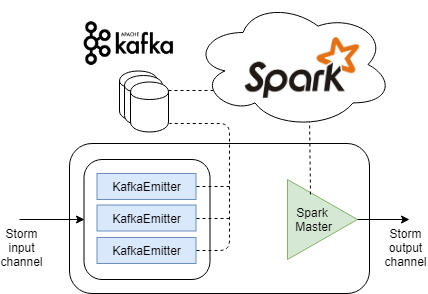
\includegraphics[width=.7\textwidth]{resources/img/distributed_accumulator.png}
\caption{Graphical depiction of the distributed accumulator process}
\label{fig:distributed_accumulator}
\end{figure}

Two interesting remarks should be made, as apparent from Figure \ref{fig:distributed_accumulator}. Firstly, The KafkaEmmitter can be replicated in order to prevent it being a point of congestion in the topology. Secondly, the fact that two distinct components (KafkaEmitter and SparkDriver) are present is encapsulated by the topology builder. Developers need only declare an implementation of the distributed accumulator processor (acting as Spark driver node) with the appropriate Storm and Kafka channels. The builder will then deploy a KafkaEmitter (or several) and the specified accumulator. This simplifies deploying the processor and obscures the internals by appearing as a single component.

\subsection{Scaffolds for micro-components}
With the high-level architecture and technologies established, the component scaffolds that are provided to application developers by the platform will be described. First, the base functions shared by all components will be described, before discussing them more in depth individually.

\subsubsection*{Common functionality}
Firstly, the components contain all functionality and information required to emit snapshots to subsequent components. A developer need only package the information in a snapshot consisting of key-value pairs and specify to which stream a snapshot must be emitted. The component then uses the information it received during the building of the topology to route the snapshot to all receivers subscribed to receive it. This not only implies routing the snapshot towards the correct component but also the correct component worker according to the defined field grouping.

Secondly, all components contain a base implementation of the \emph{prepare()} method. This method can be implemented to instantiate some properties that cannot be instantiated in the object's constructor. The reason that some properties cannot be instantiated in the constructor is that Storm processes (spouts and bolts) adhere to a prespecified execution order. The component is:
\begin{enumerate}
\nospace
\item created by one of its constructors,
\item transmitted to one of the worker nodes of the Storm cluster,
\item further instantiated using the \emph{prepare()} method, and
\item executed according to its specification.
\end{enumerate}
The reason for this course of action is that step 1 is performed on the Storm master node, before distributing the functional object over the cluster. Therefore, during step 2 the object and its members need to be serializable. Non-serializable members are consequently instantiated during step 3, after the object has been transferred and before functional execution. The \emph{prepare()} method thus can be used to instantiate certain non-serializable properties.

\subsubsection*{Spout}
This process mirrors the Apache Storm spout and is the component that introduces snapshots to the network. This component typically contains a handle to some external data source such as a database, API or auxiliary streaming technology. The reason for such a specific processor for this is the special execution cycle it has compared to a Storm bolt. Bolts execute with interrupts. They halt their execution until a new snapshot is available. However, a spout runs on an infinite-loop (until termination), continuously executing the method \emph{nextTuple()}. This method polls, retrieves and emits snapshot depending on the origin of the source.

\subsubsection*{SingleMessageProcessor}
This component is the most basic scaffold and closely resembles a Storm bolt. It however contains some additional functionality that improve its usability. It receives a snapshot and performs computations or analyses on it, before emitting new, enriched snapshots. Its typical use is for transformations of individual snapshots. As noted before, this component requires implementation of a singular method: \emph{runForMessage(Message\ m)\emph} which will be called for each snapshot received by the component.

\subsubsection*{HistoricBufferedProcessor}
The HistoricBufferedProcessor resembles the SingleMessageProcessor in that it consumes single snapshots, but instead it processes or analyses an ordered series of relevant snapshots, called a \emph{window}. This is performed by retaining an in-memory buffer to which new snapshots are amended and is periodically filtered on relevance. This component can for example be used to determine recent trends in system parameters. The methods that require implementation for this component are \emph{runForBuffer(List\textless Message\textgreater\ l)}, which is run every time the buffer is updated, and \emph{cleanBuffer(List\textless Message\textgreater\ l)} which implements how and which elements should be pruned from the buffer, should they lose their relevance.

\subsubsection{DatabaseBufferedProcessor}
From a processing perspective the DatabaseBufferedProcessor is similar to the regular HistoricBufferedProcessor. It analyses a buffer of snapshots in order to emit a snapshot containing accumulated or averaged knowledge based on its input snapshots. However, rather then keeping an in-memory buffer of snapshots it maintains a connection with an database. This allows for buffered processing of snapshots that is not performed regularly, thereby not superfluously occupying memory resources.

To keep the component applicable to many database implementations and query languages it was chosen not to instil a specific database connection. Instead, a developer is offered scaffolds to stepwise implement the intended behaviour with an actual  database connection. This scaffolding contains the methods processing the buffer (\emph{runForBuffer(List\textless Message\textgreater\ l)}) and purging the buffer (\emph{cleanBuffer(List\textless Message\textgreater\ l)}) as included in the HistoricBufferedProcessor. Aside from those functions it specifies function end-points for storing a new snapshot into the database and for fetching the relevant buffer from the database, respectively named \emph{persistMessage(Message m)} and \emph{fetchBuffer(Message m)}.	

\subsubsection{DistributedAccumulatorProcessor}
This component aggregates large amounts of laterally relevant snapshots. Laterally relevant entails that the snapshots describe similar data points, but have little sequential relevance. The input for this process is a large amount of (individually) low-information snapshots. Conversely, the goal of the processor is to emit some high-information snapshot. An example of its usage is combining thousands of snapshots from sensors in order to obtain some collective application-level performance parameters. To accomplish the aggregation of these enormous amounts of data the accumulator principle described in section \ref{sec:incorporation_spark} is employed. By means of the method \emph{runForRange(JavaRDD\textless Message\textgreater\ rdd)} this component offers implementers a reference to the Spark RDD which contains all the snapshots collected during a prespecified time period. The implementer can then use this RDD reference to sequentially manipulate and aggregate the collection of snapshots. Keeping proper parallelization in mind, this distributed component can perform data enrichment tasks on enormous batches of streaming data.

%A final remark to be made is on the granularity of the batch processing. Some real-time properties are lost by collection and processing streaming data as batches. This has been partly mitigated by employing the windowing mechanism of Apache Spark Streaming. This mechanism collects data in relatively small sub-RDDs. one or more of these smaller consecutive RDD's are then collected as one larger RDD called the 'window'. This window has a fixed size and slides over the sequence of sub-RDDs. This allows these small batches to be part of several consecutive windows. A graphical representation of this process is depicted in Figure \ref{fig:spark_window}. By this method it allows for example the analysis of data windows of the past 5 seconds, every one second. Whereas without this mechanism it would only be possible to process the last 5 seconds every 5 seconds or the last second every 1 second. Additionally, this process is very efficient, since the internal windowing mechanism automatically caches the results of the intermediary sub-RDD's. Therefore the entire chain of computations does not need to be recalculated for each windowed operation, only the transformations past the caching of the sub-results.

%\begin{figure}
%\centering
%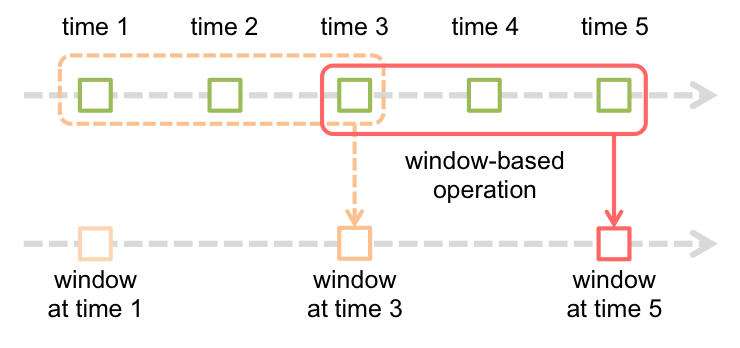
\includegraphics[scale=0.55]{resources/img/spark-window.png}
%\caption{Apache Spark windowing mechanism. Source: \cite{spark_user_guide}}
%\label{fig:spark_window}
%\end{figure}

\subsubsection*{AccumulatorProcessor}
This component closely resembles the function of the above described DistributedAccumulatorProcessor, but is executed locally rather than on a cloud cluster. The purpose of this processor is tasks that would otherwise require the distributed accumulator, but whose limited scope be run in-memory on a single worker node. This could be a viable solution for applications that either run the accumulator task often enough or do not collect excessive amounts of snapshots. For these class of applications a locally executed accumulator task should prove sufficient and inclusion of such a components eliminates the base requirement of a Apache Spark cluster to be deployed in order for the platform to be executed, since the DistributedAccumulatorProcessor is the only component that employs it. It should however be noted that not deploying an accumulator in distributed mode could introduce a bottleneck in a Storm topology since the accumulator cannot be duplicated or load-balanced.

The processor was modelled after the MapReduce paradigm \cite{mapreduce} to guide its implementation. An implementer need only specify a \emph{map}, \emph{reduce} and \emph{collect} step.  The exact methods to implement for this are:
\begin{description}[font=\normalfont]
\nospace
\item[\emph{map(Message m) : String}] \hfill \\ Computes the key for a key-value snapshots.
\item[\emph{reduce(String key, List\textless Message\textgreater\ l) : Message}] \hfill \\ Reduces sets of key-value pairs grouped by key determined in the map step.
\item[\emph{collect(Map\textless String,Message\textgreater\ m) : Map\textless String,Message\textgreater}] \hfill \\ Collects the key-message pairs emitted by a reduce step. The return value of this method is a map of snapshots indexed by the Storm topic on which it should be forwarded.
\end{description}
Please note that the result of the reduce step is a set of snapshots. It is therefore possible to chain multiple map-reduce steps sequentially, as long as the sequence is concluded with a single collect step.

\subsubsection*{ResourceDistributionModelProcessor}
The final component is the ResourceDistributionModelProcessor. This processor is a special instantiation of the SingleMessageProcessor that analyses inbound snapshots according to a prespecified Resource Distribution Model (RDM). This model will be discussed in detail in Chapter \ref{ch:rdm}. In contrast to all other processors, this processor is not just a scaffold. Instead, it executes completely automatically, requiring only an instantiation of an RDM and a specification of which model variables to output on which Storm channels. The processor then automatically provisions the input variables of the model, calculates the derived values and outputs the requested values as specified.

\section{Demonstration by example case}
\label{sec:example_application_topology}
This section will demonstrate an example of a composition of the specified components to a hypothetical WSN application. First, the hypothetical example case used in this chapter (and the next) will be described shortly. Following, the platform will be explained according to a hypothetical application to that case.

\subsection{The example case}
\label{sec:example_case}
Before describing the example case, some context must be given. This case may sometimes seem oversimplified and nonsensical, but it does provide an elementary example to illustrate all facets of the solutions without overcomplicating the case. This case is expressly not intended to demonstrate the validity or utility of the proposed solutions. For that purpose, an application to a more complex real-world case will be performed in Section \ref{ch:validation}

The proposed case encompasses an enormous network of low power devices sensing for meteorologically anomalous events. These sensors perform measurements on a regular interval and transmit the measurements to a cell tower to be forward to a back-end application for further processing. For the best results devices should measure and transmit as much as possible. However, since these sensors are not very powerful and employ a limited power supply they will require pacing.

The behaviour of the sensors is typified by two parameters: the sensing interval and transmission interval. Intuitively, it can be stated that shortening either or both of the intervals will result in more fine grained reporting, but will increase the power consumption of the device. Additionally, over time several types of sensors have been deployed with different power sources. Therefore, a sensor's power consumption over a given time needs to be restrained in accordance with the specification of its power source and expected life-time. Additionally, sensors in areas of high interest will require a shorter polling interval, as instructed by the back-end application, to gain the most precise information. Finally, given that the sensor performs the adequate amount of measurements and does not consume more power than it is specified to use, it should measure and report as much as permitted.

As for what requires monitoring, the most interesting metric is the measurement rate averaged over all sensors. Additionally, it is required to pro-actively monitor the trend of the total bandwidth used by the sensor application. The reason for this is that a constant rise in data rates may ultimately violate the data rate limits agreed upon with network service providers.

To summarize, a sensor must:
\begin{itemize}
\nospace
\item not consume more power then it is allowed according to its battery specification,
\item measure at least as much as is specified according to the area of interest it is in, and
\item generally try to measure and report as much as is allowed by the previous two requirements.
\end{itemize}
Additionally, the following information must be reported by the application:
\begin{itemize}
\nospace
\item The average polling rate, and
\item whether the data rate of the sensor application rises consistently for a certain amount of time.
\end{itemize}

In order for the server to determine the intended behaviour of the device and calculate the level of service provided by the application, the following data regarding a sensor device is provided to the monitoring application:
\begin{itemize}
\nospace
\item the required measurement rate,
\item the maximum power provided by the power source,
\item the measurement rate of the sensor device, and
\item the bandwidth used by the sensor
\end{itemize}
Each of these data points stipulates the behaviour of a single sensor at a certain instant. Notice that some data points are normally inferred from raw basic data by auxiliary processes (e.g. required measurement rate). For simplification of the demonstrations these processes are omitted and these parameters are presumed known as a message is introduced into the monitoring application.

\subsection{Application of the platform}
\begin{sidewaysfigure}
\centering
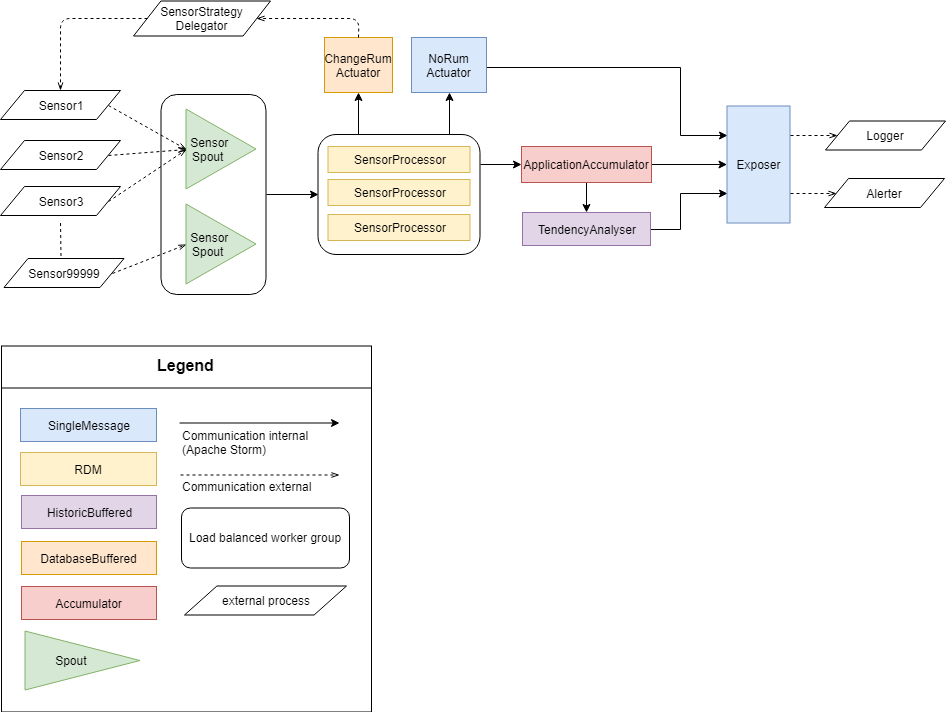
\includegraphics[width=\textwidth]{resources/img/example_topology.png}
\caption{Example topology of a platform implementation according to the example case}
\label{fig:example_topology}
\end{sidewaysfigure}
A graphical representation of the topology for the example implementation is depicted in figure \ref{fig:example_topology}. As the figure makes apparent, the application encompasses a large number of sensor devices. These devices regularly send their status information to the monitoring application via some external communication technology (e.g. Apache Kafka). These snapshots are introduced into the topology by \emph{SensorSpouts}. These spouts have been duplicated in order to accommodate the large amount of sensors which might send a sudden burst of data. The snapshots are then forwarded to the \emph{SensorProcessors} which have been provisioned with a Resource Distribution Model. This model consumes the measured parameters of the input snapshot and uses them to further calculate all the parameters which can be derived from the inputs, according to the specified model. This model also determines the optimal Resource Utilization Model (RUM) for this sensor device. Should no valid model composition be found this is reported to the \emph{NoRumActuator} which forwards a log message to the \emph{Reporter} component. The \emph{Reporter} will delegate the message to the correct reporting/alerting mechanism, outside of the topology.

Should the current mode of operation be determined not to be optimal, the \emph{SensorProcessor} will report to the \emph{ChangeRumActuator}. The \emph{ChangeRumActuator} will report requests for change to an entity outside of the topology of the application. The actuator has been implemented as a DatabaseHistoricProcessor. The reason for this is that it will recollect the last few snapshots it received for this sensor and will only actually change the mode of operation of the sensor if it is consistent with the last few snapshots received. This eliminates superfluous communication with the sensor device caused by sporadic behaviour. Alternatively, this component could have been implemented as a BufferedHistoricProcessor. However, a sensor is expected to send monitoring data only a few times per day and changes of operation will occur even less. It would therefore make little sense to keep a buffer of the last snapshots sent for each and every sensor in-memory. Additionally, this would have required a field grouping in case the component were to be load-balanced in order to enforce that the request for change of a particular sensor always be sent to the correct worker.

The final transformation to be performed is to infer application-level intelligence from the low-level sensor statuses. This is performed by the ApplicationAccumulator which collects data for a certain time period and calculates some high-level data points, such as the measurement rate of the application averaged over its sensors, the total throughput and how many devices are performing on which RDM. This information is forwarded to the \emph{Reporter} which will make it available for visualization performed outside of the topology. Additionally, the accumulator sends its aggregated snapshot to a \emph{TendencyAnalyser} which keeps a sequence of the total bandwidth used during previous time windows. Should this total consistently rise over a period of time, an alert will be sent by the reporter, as specified by the alerting requirements listed in section \ref{sec:example_case}.
	
\section{Discussion of the proposed software platform}
This section will evaluate the design of the monitoring platform.

\subsubsection*{Satisfaction of requirements}
The first order of business is whether the proposed design satisfies the earlier stated requirements. The message-passing micro-component architecture provides the basis for snapshot transferral and transformation as stated in requirement \ref{r:snaptshot_transformation}. Furthermore, the requirements \ref{r:basis_single}, \ref{r:basis_historic} and \ref{r:basis_accumulated} are satisfied by the inclusion of the \emph{SingleMessageProcessor}, \emph{BufferedProcessors} and \emph{AccumulatorProcessors}, respectively. Finally, the last two requirements regarding the size of the applications in the problem domain and entailing scalability of the solution have been decisive for certain choices of the supporting technologies. For example, it is reflected in the employment of cloud processing technology Apache Spark. From the aforementioned arguments it is concluded that every requirement is represented and met in the design of the platform.

\subsubsection*{Completeness with respect to QoI attributes}
The goal of the platform is to process and enrich data. It is therefore rational to evaluate the appropriateness and completeness of the platform by considering the information processing capabilities it offers. This section thusly evaluates the platform's completeness by demonstrating that the platform only positively impact the Quality of Information (QoI) of the input data. This entails that the QoI is improved or retained, but never lost as data passes through a platforms topology. This will be achieved by arguing the QoI parameters which were enumerated in Section \ref{sec:back:qoi} of the Background.

The first consideration of QoI is regarding the processing of data by the platform and affects the precision, completeness and usability of information. Firstly, \emph{precision} and \emph{certainty} are obtained by employing the HistoricProcessors. By averaging measurements, anomalies are mitigated and the reported value closely approaches the norm of the measurements. Provided that the accuracy of the measurements is sufficient, this improved precision should consistently yield a measurement near the actual value. Secondly, the \emph{Usability} of information is improved as data moves throughout the topology. To illustrate this a thought experiment is proposed, using the example topology listed and described in section \ref{sec:example_application_topology} and a batch of raw data emitted during a certain time window. Before the data enters the platform it contains the potential to calculate the average throughput offered by the sensor application during that time window. However, this data point is not present explicitly. This process is performed by an implementation of the platform and the resulting information is offered for further processing or visualization. This demonstrates that the platform can facilitate usability for information by calculating and producing ready-for-use values. It should however be noted that the \emph{completeness} of the information is greatly reduced during this process. To illustrate, from the average application throughput the throughput for individual devices can no longer be determined. For this reason, and others which will become apparent, committing the raw data to storage before processing is recommended.

The second class of QoI attributes regards the processing efforts, expressed in time and costs. As the relevance of information degrades as time progresses, timely processing is paramount. \emph{Timely} execution is achieved by providing a scalable distributed solution. This ensures that, regardless of the intense information \emph{throughput}, the calculations can be performed in near real-time. Notice that only near real-time is claimed, since Apache Spark collects records during a time window and performs calculations in batches. However, the time window of such a batch can be set arbitrarily small for fine-grained processing. Thereby it does not impact the timeliness significantly. However, adverse to this gained timeliness is a decreased \emph{affordability}. In order to incorporate these distributed cloud technologies a cluster of machines and increased development resources will need allocation. When the solution does not require this degree of scalability this poses an undue burden. Therefore, locally deployable alternatives to these distributed processors are also provided. Implementations of the platform are therefore offered a trade-off between timeliness and cost.
	
Lastly, are the \emph{tuneability} and \emph{reuseability} of the information. Firstly, the data can be duplicated among different communication channels which allows differentiating calculations to be performed on the same data. Secondly, in order to facilitate evolution of end-user demands the platform has been designed with separation of concerns in mind. This allows continuous reconfiguration of the platform to be performed with reduced occurrence of concern entanglement. By redeploying the topology the same raw information can be used to facilitate updated user demands. This is also another reason to store the raw data before processing it.
%By caching the data it can be re-fed into an updated topology in order to initialize an application as if it had been running for days.

Some final remarks should be made on the analysis. Firstly, the platform cannot offer any improvement or retention of information \emph{accuracy}, as it is solely determined by the method and quality of data measurement. Secondly, it should be noted that the platform does not assure preservation of any of these claim, since an implementation of the platform can violate any guarantee made. It can only be claimed that the platform does not impede any of the parameters and offers the means for developers to develop applications that do guarantee it.

\subsubsection*{Ease of adoption}
A second point of focus is the ease of adoption provided by the platform itself. It is asserted that low-level implementation details of Apache Storm and Spark are effectively obscured. This was achieved by offering some abstract components that require implementation of only a few methods. This obscuration entails a clearer programming interface to an implementer, as stated by the fa\c{c}ade software design pattern \cite{facade_pattern}

Secondly, the provided topology builder facilitates easy and fast building of a Storm topology. It does so by providing context-aware topology and process instantiation, and topic based communication subscription and emission.  As mentioned before this allows $M$ producers and $N$ consumers connected by a single topic to be connected with complexity $\Theta(M+N)$, instead of the complexity $\Theta(M\cdot N)$ which would be required without the concept of topics. These assertions will be formally validated in Chapter \ref{ch:validation}.

\subsubsection*{Technology stack}
Another issue to contemplate is the technology stack required for the platform. As mentioned in section \ref{sec:solution_decision}, Apache Storm was chosen as chief enabling technology. The main reason for this is that it offered most of the features required and would reduce the technology stack. However, by employing Apache Spark for distributed data aggregation, two additional cloud technologies are introduced. Spark itself and Kafka which is required in order to be connected to a Storm topology. However, the inclusion of a distributed aggregation is necessary in order to keep the computations scalable. Additionally, the speed and efficiency arguments raised in section \ref{sec:solution_decision} justify the deployment of these additional technologies. Finally, when this scalability is not required Apache Spark and Kafka clusters can be executed locally on a single machine. This would still enjoy benefits from process parallelization, without requiring cluster deployment. Finally, Spark and Kafka may be omitted entirely, if permitted by the snapshot influx, as a non-distributed accumulator is also included in the platform.

%\subsubsection*{Future work}
%Finally, the topology-based separation of concern approach allows for visualization of the computations and distribution. The chain of computations can easily be depicted as a directed graph with processors and topics as nodes and processor-topic connections as vertices. Such a topology visualization would for example be very useful for identifying incorrectly or disconnected components. While runtime analysis tools are available for Storm topologies a graphical modelling/development tool is lacking. Such a tool would allow a topology to be drawn and functional methods to be implemented later. Though not featured, future efforts could be made to facilitate them.

%ease of use
%large technology stack
%qoi metrics
	%datastreams


%ease of use
%	topology build by 2 lines of code per component (4 if formatted)
%		create, register, declare, subscribe
%	total for test topology = xxx
	
%large stack -> also supply old accumulator
%also supply old
%		lower stack
%		gebruikt during development
%		map-reduce
%			rdd not map-reduce
%		Spark can run locally
%???	
%1. Every stream ends in distinct collection/number of streams -> therfore no n*m analysis necessary (only for each stream and for each analysis individually. (htis only descirbes outputs, not the inputs)
%2. there are no one/N to many relations. Implications?
%+RUM

%no mass emitter?
%??


%Discussion aan de hand van qoi metrics

%future work?
%composer GUI?



%architecture
%	model reification
%what components needed
%	featuremodel
%	requirements
%which candidates
%benchmarking
%desicions
